\documentclass[letterpaper,12pt]{article}

% IMPORT PACKAGES
\usepackage{amsmath, amsfonts, amssymb, amsthm}		% math equations
\usepackage{commath}								% more math equations
\usepackage{ifthen}									% conditional statements
\usepackage{pgfplots}
\usepackage{calc}  
\usepackage{tikz}
\usepackage{fancyhdr}
\usepackage[shortlabels]{enumitem}					% use letters to enumerate
\usepackage[english]{babel} 						% language-based hyphenation
\usepackage{blindtext}								% example text
\usepackage{microtype}								% improve justification
\usepackage{wrapfig}								% wraps words around figures
\usepackage{enumitem}								% improve lists
\usepackage{index}									% indices
\usepackage{lastpage}
\usepackage{extramarks}
\usepackage[plain]{algorithm}
\usepackage{algpseudocode}
\usepackage{matlab-prettifier}
\usepackage{verbatim}
\usepackage{fancyvrb}
\usepackage{actuarialsymbol}
\usepackage{indentfirst}
\makeindex
\pgfplotsset{width = 9.5cm}
\pgfplotsset{compat=1.5}

\usepackage{graphicx}								% use pictures
\graphicspath{ {./out/} }

\usepackage{hyperref}								% hyperlinks
\hypersetup{
    colorlinks=true,
    linkcolor=black,
    filecolor=magenta,      
    urlcolor=cyan,
    pdfpagemode=FullScreen,
    }

\usetikzlibrary{automata,positioning}

% CHANGE PAGE MARGINS
\usepackage[letterpaper, inner=1in, outer=1in, top=1in, bottom=1in, bindingoffset=0in]{geometry}

% CHANGE FONT
\usepackage{mathpple}
\usepackage{dsfont,listings}
%\usepackage{lmodern}
%\usepackage[T1]{fontenc}
%\usepackage{mathptmx}
%\usepackage[textwidth=6.5in, textheight=9in]{geometry}

% HEADER/FOOTER
\pagestyle{fancy}
\fancyhf{}
\setlength{\headheight}{28pt}
\lhead{\Class \\ \Title}
\rhead{\AuthorName \\ \ClassInstructor}
\cfoot{\thepage\ of \pageref{LastPage} }

% TITLE PAGE
\title{
    \vspace{2in}
    \textmd{\textbf{\Class:\ \\ \Title}}\\
    \vspace{3in}
}
    \author{\AuthorName \vspace{2pt}\\ \textit{\ClassInstructor}}
	\date{}

% CUSTOM GLOBAL COMMANDS
\newcommand{\Title}{Beginning Scientific Computing}
\newcommand{\Date}{May 7th, 2023}
\newcommand{\Class}{Learning MATLAB}
\newcommand{\ClassInstructor}{Professor Tae Eun Kim}
\newcommand{\AuthorName}{Ian McCamey}

\newcommand{\alg}[1]{\textsc{\bfseries \footnotesize #1}}
\newcommand{\deriv}[1]{\frac{\mathrm{d}}{\mathrm{d}x} (#1)}
\newcommand{\pderiv}[2]{\frac{\partial}{\partial #1} (#2)}
\newcommand{\E}{\mathrm{E}}
\newcommand{\Var}{\mathrm{Var}}
\newcommand{\Cov}{\mathrm{Cov}}
\newcommand{\Bias}{\mathrm{Bias}}
\def\code#1{\texttt{#1}}

\begin{document}
\maketitle
\pagebreak

\section*{Introduction}

This report contains an overview of my work in completing MATH 3607, Beginning Scientific Computing, a course specializing in the programming and numeric computing platform MATLAB at The Ohio State University during the Spring of 2023.  The course was designed as an introduction to the mathematical theory of algorithms used to solve problems that typically arise in sciences, engineering, and finance.  Specifically, several key concepts taught in this course are applicable to the main responsibilities of actuaries, data scientists, and other quantitative thinkers. 

My purpose in presenting this document publicly is to showcase my experience in utilizing statistical software to solve complex mathematical problems via numerical computations.  In addition, given the complexity of the mathematics involved, I hope to reduce each problem into a digestible form for a non-technical reader to understand, as this kind of conceptual simiplification is necessary when communicating with others in the professional world.

It is worthy to note that the programming language R is more commonly used in the actuarial profession for data-driven calculations and analysis. However, it and MATLAB share many commonalities. In particular, both
\begin{itemize}
	\item are used for numerical computations,
	\item support functional programming,
	\item support array programming (vectorized operations),
	\item allow plotting of functions and data, and
	\item allow implementation of algorithms.
\end{itemize}

As to where they differ, an experienced programmer knows that their syntactical differences are minor compared to their conceptual similarities.  However, R admittedly has a greater ability to handle and manipulate large datasets, while MATLAB can apply the theories of linear algebra far better than R.  A near-comprehensive comparison between the two languages can be found \href{https://cran.r-project.org/doc/contrib/Hiebeler-matlabR.pdf}{here} in a PDF from the University of Maine.

Let's begin to see how MATLAB can be used to gain insight about the nature of our world through mathematical models and computation.

\pagebreak

\subsection*{Annuities}
A basic type of investment is an annuity: one makes monthly deposits of size $P$ for $n$ months at a fixed annual effective interest rate $i$, and at maturity collects the amount
$$ F = P \ax{\angln i} = P \left(\frac{(1+i)^n - 1}{i}\right). $$ 
Say you want to create an annuity for a term of $300$ months and final value of \$1,000,000. Using MATLAB, you can make a table of the interest rate you will need to get for each of the different contribution values $P = 500, 550, \dots , 1000$. Implementing this into code, we can write the following which prints to the console:
\\
\begin{lstlisting}[
frame=single,
style=Matlab-editor]
n = 300;
F = 1000000;

for P = 500:50:1000
    if P == 500
        fprintf(' %10s %12s\n', 'Payment, P', 'Rate, r')
        fprintf(' %25s\n', repmat('-', 1, 25))
    end
    % function definition
    f = @(i) P*((1 + i)^n - 1)/i - S;	
    % finding roots
    i = fzero(f, [eps 1]);
    fprintf(' %10d %12.6f\n', P, i)
end
\end{lstlisting}
\VerbatimInput{out/out01.txt}

\pagebreak

\subsection*{Random Walks}
In a computer, data is stored as a finite number of bits. Therefore, not every number can be stored \textit{exactly}; there is a small error between the number and its computer-based (floating point) representation.  It’s reasonable to expect, then, that floating point errors accumulate randomly during a long computation. 

On average we expect as many errors to be negative as positive, so they tend to partially cancel out. In fact, a classical result of probability is that, as the number of computations increases, the average of all of these random errors is very near $0$.

Here is a plot of 50 simulations of this randomly compounding error in MATLAB.

\begin{lstlisting}[
frame=single,
style=Matlab-editor]
clf
rng(6960)
n = 10000;
n_walks = 50;

for i = 1:n_walks
    % generate random errors
    r = randn(n,1); 
    % accumulate errors
    y = cumsum(sign(r));	
    plot(y(1:5:end)), hold on
end
title('50 Random Walks')
\end{lstlisting}
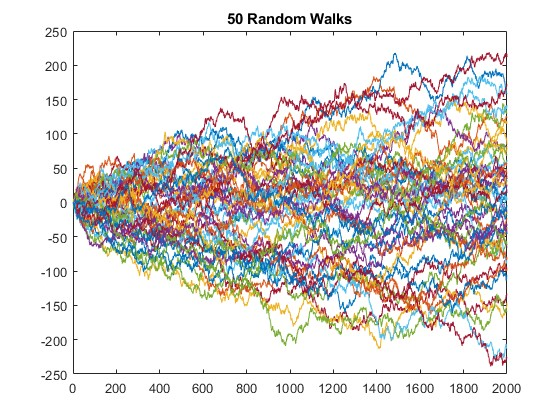
\includegraphics[scale=0.7]{random_walks}

\subsection*{Stock Price Simulation}
Remember that continuously compounding interest can be expressed by (an equation 
familiar to most)
$$P = e^{rT}$$
Alternatively, this can be rewritten as
$$S(T) = S(0) e^{rT}$$
where $S(0)$ is the initial balance of the account, $r$ is the continously 
compounding annual interest rate, $T$ is the total time in years, and $S(T)$ 
is the account balance after $T$ years. This is useful when computing the future 
value of something like a savings account or a bond.

However, if we wanted to model something more complicated, such as the price 
of a share of stock, we can instead imagine that our initial balance might increase 
or decrease randomly over time. As a starting point, we can conceptualize these 
random price movements as a series of coin flips: our account balance $S(0)$ 
is multiplied by a factor of $e^{rT}$ if we land on heads, and it is divided 
by a factor of $e^{rT}$ if we land on tails. "Flipping the coin" many times 
creates an up \& down, alternating sequence of account balances that look similar 
to the value of shares in stock.

As it turns out, this model can be improved to better reflect reality. In 
particular, real stock prices generally tend upwards over time. For instance, 
the S\&P 500 has a return on investment of 9.75\% per year since 1930. The simplest 
way of introducing this into the model is to make our "heads" factor slightly 
greater than our "tails" factor, so that the average change resulting from a 
single coin flip is net positive. 

As an example, we may, for each "heads" or "tails," multiply or divide by 
$e^{rT}$as before, but in either case we will always multiply by some other 
factor $e^{\alpha T}$ where $\alpha < r$.

In one specific model, the Black-Scholes-Merton (BSM) model of stock prices, 
the term in the exponent is, instead of a flat interest rate $rT$, converted 
to reference real historical data of the stock's performance. It captures how 
one might expect a stock to change in value given certain facts about its history.

In essence, the BSM model attempts to actually reflect the particular stock 
in question, taking into account things like expected rate of return on investment 
$\alpha$, the dividend rate $\delta$, and the volatility $\sigma$ of the stock 
in question. 

In this model, our term in the exponential (instead of $rT$) is defined by
$$\left(\alpha - \delta - \frac{\sigma ^2}{2} \right)T \pm \sigma\sqrt{T}$$
While this is intimidating, it's important to note that $\left(\alpha - \delta 
- \frac{\sigma ^2}{2} \right)T$ is our component which reflects the "upward 
drift" in stock prices over time, and we add or subtract $\sigma\sqrt{T}$ from 
this for a "heads" or "tails" result, respectively. In summary, our stock price 
balance is found in the BSM model by
$$S(T) = S(0) e^{\left(\alpha - \delta - \frac{\sigma ^2}{2} \right)T \pm \sigma\sqrt{T}}$$
We can further improve by converting our "heads" and "tails" factors $\pm\sigma\sqrt{T}$ 
into something that represents more outcomes than those of a simple "coin flip." 
We can do this by taking $\sigma\sqrt{T}$ and multplying it by a random number 
that could be positive or negative; in this way, we can randomly "scale" how 
much our stock goes up or down, allowing for bigger or smaller "jumps" in price. 
We can implement this additional "randomness" into our model by writing
$$S(T) = S(0) e^{\left(\alpha - \delta - \frac{\sigma ^2}{2} \right)T + \sigma\sqrt{T}Z}$$
Here, $Z$ represents a random number that could be positive or negative. Put 
plainly, the value of $Z$ could theoretically be any number between $-\infty$ 
and $\infty$, but is most likely (99.7% chance) to be somewhere between -3 and 
3. More technically, $Z$ follows a standard normal distribution $\mathcal{N}(0,1)$. 
The standard normal distribution $\mathcal{N}(0,1)$ is a common and well-documented 
statistical concept that is widely used in probability theory, and we can use 
this to our advantage in stock pricing.

This is our primary equation that we will use in this code to carry out calculations. 
In particular, we will use the above equation to model prices of stock given 
various input parameters. We will then compute the probabilities that our stock 
will be above or below certain hand-chosen prices. 

We will then compute the premium of call and put options derived from the 
simulated stock using the Black-Scholes formula. We will show that our $\Delta$ 
value found by the formula is equivalent to the corresponding probabilities 
that our stock will be above or below the chosen strike prices.

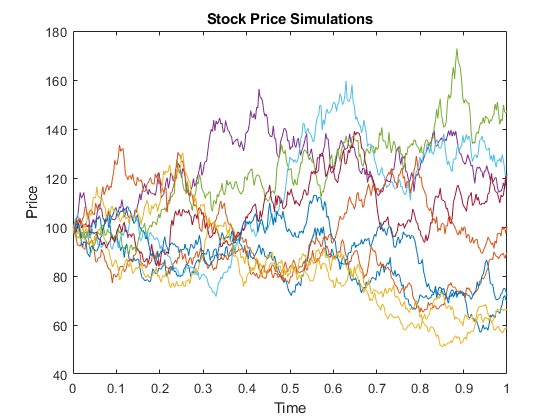
\includegraphics[scale=0.8]{stock_sims}
\begin{lstlisting}[
frame=single,
style=Matlab-editor]
% INPUT PARAMATERS:
%   n_sims: number of simulations
%   T:      number of years in each simulation
%   n:      number of periods in each simulation
%   S_t:    stock price at time t
%   r:      annual continuous risk-free rate of return
%   alpha:  annual continuous rate of return
%   delta:  annual continuous dividend rate
%   sigma:  annual volatility of stock prices

n_sims  = 10;
T       = 1;
n       = 365;
S_0     = 100;
r       = 0.05;
alpha   = 0.05;
delta   = 0.01;
sigma   = 0.4;

% COMPUTING STOCK PRICES
rng(1000);
h = T/n;
% preallocate array of stock prices
S_t = zeros(n, n_sims);
% random numbers to scale up & down factors
z = randn(n, n_sims);
t = linspace(0, T, n);
a = (alpha - delta - sigma^2 / 2) * h;
b = sigma * sqrt(h);

for i = 1:n_sims
    S_t(1, i) = S_0;
    for k = 2:n
        S_t(k, i) = S_t(k-1, i) * exp(a + b * z(k, i));
    end
    plot(t, S_t(:, i))
    hold on
end
title('Stock Price Simulations'), 
xlabel('Time'), ylabel('Price')
hold off
\end{lstlisting}

\subsection*{Stock Price Statisics}
Using market conditions $\alpha$, $\delta$,and $\sigma$, we have simulated stock prices over $T$ years. Allowing the number of simulations to grow larger can give insight as to how the stock prices are distributed statistically.

We will now use the probability distribution of stock prices $S(t)$, the lognormal 
distribution, to discuss the chances that our stock will be above or below certain 
hand-chosen prices $k$. In particular, we will discuss $\mathbb{P} (S(T) \leq k)$ and $\mathbb{P} (S(T) \geq k)$. \\

\begin{lstlisting}[
frame=single,
style=Matlab-editor]
% COMPUTING PROBABILITIES
% array of prices from 1 to 2*S(0)
k = (1:2*S_0)';
% normal variable transformation of S(t)
d1 = (log(S_0./k) + a)/(sigma*sqrt(T))';
d2 = d1 - sigma*sqrt(T);
p_d1 = normcdf(d1);
p_d2 = normcdf(d2);          % probability S(t) > k
probs = [k, p_d2, 1 - p_d2]; % array concatenation

plot(probs(:,1), probs(:,2), 'k', probs(:,1), probs(:, 3), 'r')
title('Likelihoods of Ranges of Stock Prices'),
xlabel('k'), ylabel('Probabilities'), 
legend('P(S>k)', 'P(S<k)')
\end{lstlisting}
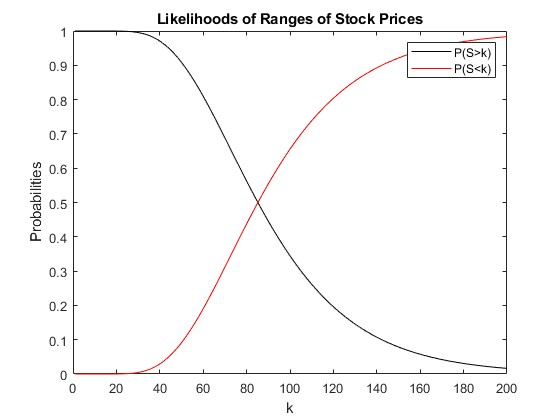
\includegraphics[scale=0.725]{likelihoods}

\pagebreak
\subsection*{Put \& Call Option Prices}
\begin{lstlisting}[
frame=single,
style=Matlab-editor]
% COMPUTING CALL & PUT OPTION PREMIUMS
C =   S_0 * exp(-delta * T) * p_d1       
    - k * exp(-r * T) .* p_d2;
P = - S_0 * exp(-delta * T) * (1 - p_d1) 
    + k * exp(-r * T) .* (1 - p_d2);
options = [k, C, P];

plot(k, C, 'k', k, P, 'r');
title('Call and Put Premiums of Different Strikes'), 
xlabel('k'), ylabel('C, P'), 
legend('Call premiums', 'Put premiums')
\end{lstlisting}
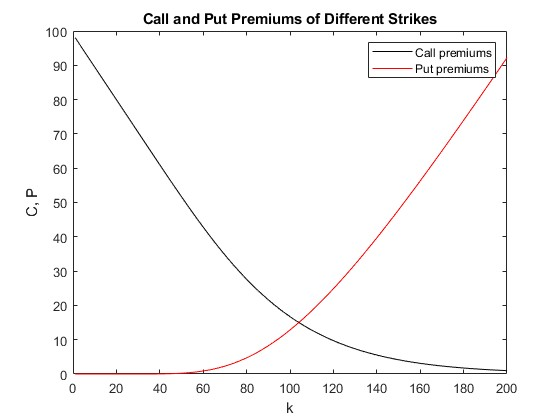
\includegraphics[scale=0.8]{premiums}

\begin{lstlisting}[
frame=single,
style=Matlab-editor]
% COMPUTING EQUILIBRIUM STRIKE AND ITS PREMIUM
% (the strike k' where call and put premiums are equal)
k_prime = S_0 * exp(r - delta)
d1_prime = (log(S_0 / k_prime) + a) / (sigma * sqrt(T));    
d2_prime = d1_prime - sigma * sqrt(T);
CP_prime = S_0 * exp(-delta * T) 
           * (normcdf(d1_prime) - normcdf(d2_prime))
\end{lstlisting}

\begin{lstlisting}[
frame=single,
style=Matlab-editor]
% OVERLAYING OPTION PREMIUMS AND PROBABILITIES 
clf
yyaxis left
plot(k, probs(:,2), 'k-', k, probs(:, 3), 'r-');
yyaxis right
plot(k, C, 'k--', k, P, 'r--');

yyaxis left
title('Premiums & Probabilities')
xlabel('Strikes')
ylabel('Probabilties')
yyaxis right
ylabel('Option Premiums')

legend('P(S>k)', 'P(S<k)', 'Call premiums', 'Put premiums')
legend("Position",[0.7,0.75,0.1805,0.175])
\end{lstlisting}
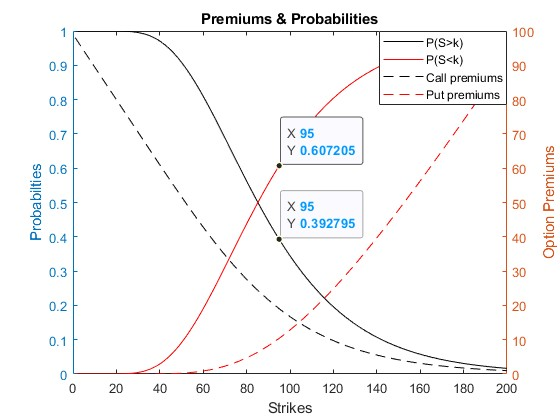
\includegraphics[scale=0.8]{premiums_probabilities}
\pagebreak

Our risk profile is better for strikes where the premium of a call/put is 
cheaper than its alternative put/call, but the stock is more likely to be above/below 
the same strike than the alternative.  For instance. for the strike $k = 95$, 

$$\mathbb{P}(S(t) < 95)  >  \mathbb{P}(S(t) > 95)$$    

However,

$$P_{95} < C_{95}$$

In other words, the put is more likely to be in-the-money than the associated 
call, but its premium is cheaper!  We are able to purchase "more chance" (and 
therefore less risk) per dollar with the put option for strike $k = \$95$.

From the above visual, we can see that this idea holds for all $k$ values 
between the intersection of the solid lines and the intersection of the dashed 
lines, or the interval $k \in \left(S_0e^{r-\delta-\frac{\sigma^2}{2}}, S_0e^{r-\delta}\right)$.

\end{document}